%!TEX root = ../../Main.tex

\section{Задача 1}
\frame{\sectionpage}
\begin{frame}{Формулювання}

		Задача

		\begin{equation}\label{eq:problem1}
		\begin{cases}
			- \Delta u(x_1,x_2) + 1000u(x_1, x_2) = f(x_1,x_2), \\
			f(x_1,x_2) = (18 \pi^2 +1000)\sin(3 \pi x_1) \sin (3 \pi x_2), \\
			u|_\Gamma = 0 ,\\
			\Omega = \left[0;1\right] \times \left[0;1\right].
		\end{cases}
		\end{equation}

		Точний розв'язок
		\begin{equation}
			u(x_1,x_2) = \sin(3 \pi x_1) \sin (3 \pi x_2)
		\end{equation}

\end{frame}

\begin{frame}{Точний розв'язок}
		\begin{figure}[H]
			\centering
		    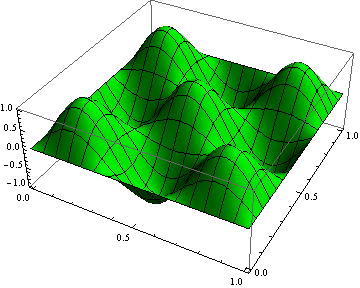
\includegraphics[scale=0.6]{problem1/ExactSolution}
		    \label{plot:problem1_exact}
		\end{figure}
\end{frame}

\begin{frame}[allowframebreaks]
	\frametitle<presentation>{Наближення}

	Граничну точність апроксимації на скінченному елементі - 5\%.

	Початкове розбиття - рівномірне на сітці 10x10
	%%
	\begin{figure}[H]
		\centering
	    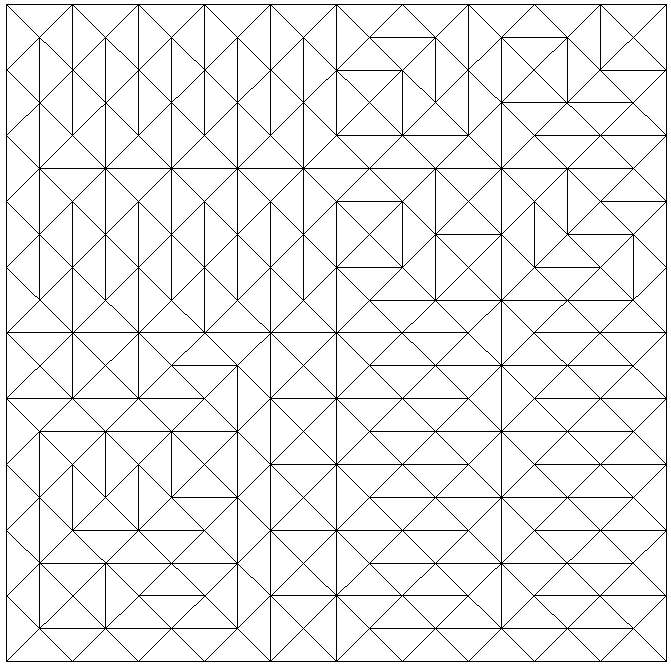
\includegraphics[width=0.4\textwidth]{problem1/InitialMesh}
	    \label{fig:init_mesh1}
	\end{figure}

	\framebreak

	Для отримання похибки в 5\% знадобилося 18 кроків та \nn{19322} скінченних елементи.

	Графіки наближень:

		\begin{figure}[H]
			 \begin{columns}
			 	\begin{column}{0.5\textwidth}
		     		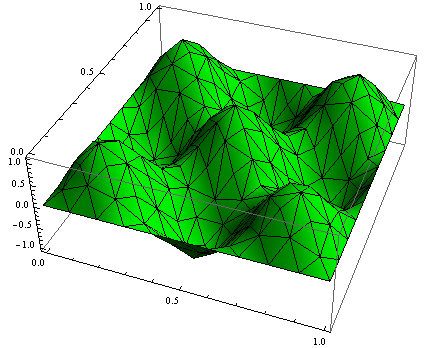
\includegraphics[width=\textwidth]{problem1/my/solutions/1}
		     	\end{column}
		     	\begin{column}{0.3\textwidth}
		     		\caption*{1-й крок. $N(h) = \nn{400}$.}
		     	\end{column}
		     \end{columns}
		\end{figure}
		%
		\begin{figure}[H]
			\begin{columns}
			 	\begin{column}{0.7\textwidth}
			 		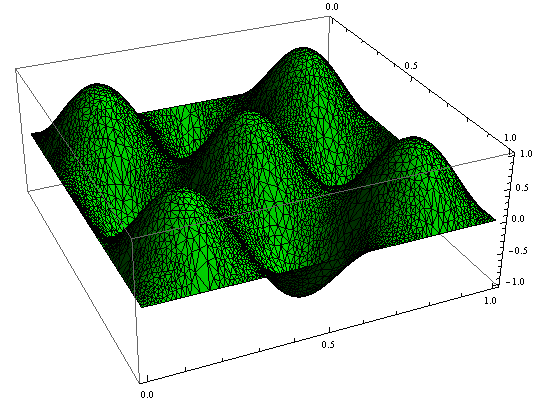
\includegraphics[width=\textwidth]{problem1/my/solutions/5}
			 	 \end{column}
			     \begin{column}{0.3\textwidth}
			     	\caption*{5-й крок. $N(h) = \nn{12903}$.}
			     \end{column}
		     \end{columns}
		\end{figure}
		%
		\begin{figure}[H]
			\begin{columns}
			 	\begin{column}{0.7\textwidth}
			 		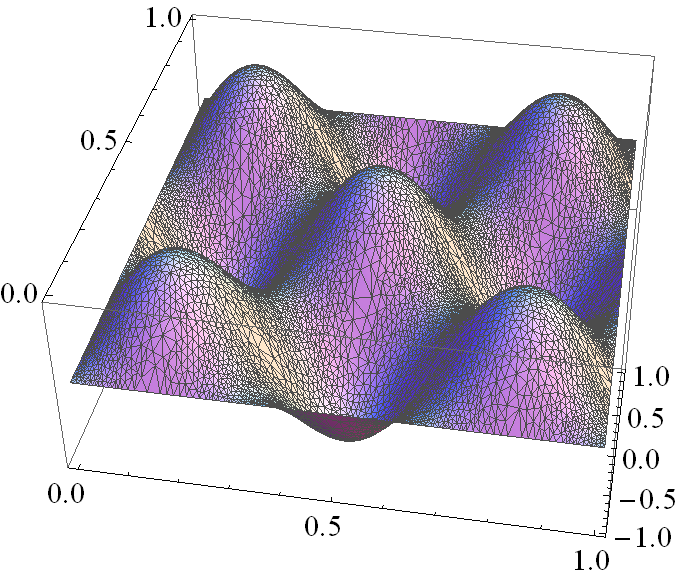
\includegraphics[width=\textwidth]{problem1/my/solutions/18}
			 	 \end{column}
			     \begin{column}{0.3\textwidth}
			     	\caption*{18-й крок. $N(h) = \nn{19322}$.}
			     \end{column}
		     \end{columns}
		\end{figure}
\end{frame}


\begin{frame}[allowframebreaks]
	\frametitle<presentation>{Індикатори похибок}
		Графіки індикаторів похибок на скінченних елементах.
		%
		\begin{figure}[H]
			\begin{columns}
			 	\begin{column}{0.5\textwidth}
			 		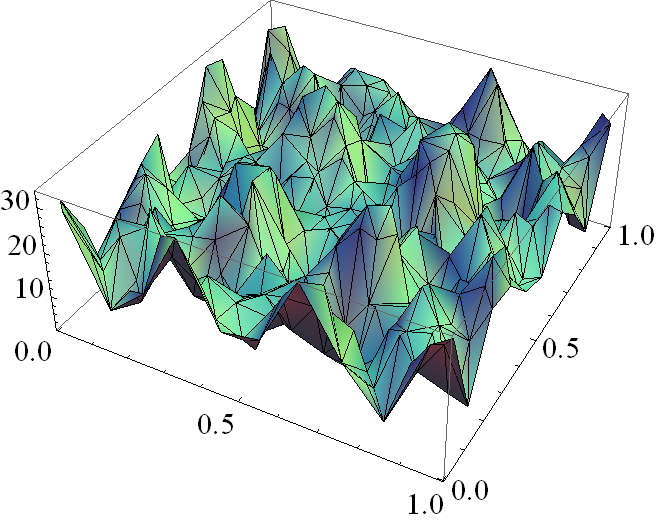
\includegraphics[width=\textwidth]{problem1/my/AEE/1}
			 	 \end{column}
			     \begin{column}{0.3\textwidth}
			     	\caption*{1-й крок. $N(h) = \nn{400}$.}
			     \end{column}
		     \end{columns}
		\end{figure}

		\begin{figure}[H]
			\begin{columns}
			 	\begin{column}{0.7\textwidth}
			 		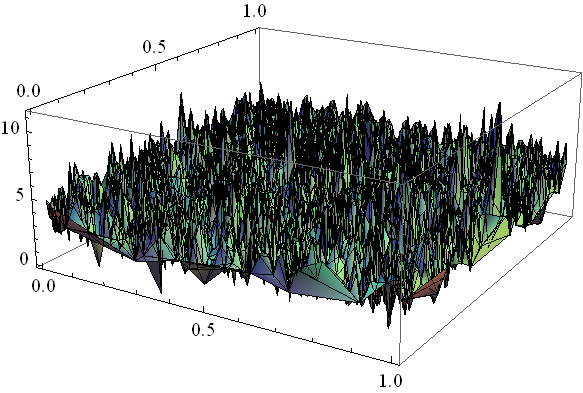
\includegraphics[width=\textwidth]{problem1/my/AEE/5}
			 	 \end{column}
			     \begin{column}{0.3\textwidth}
			     	\caption*{5-й крок. $N(h) = \nn{12903}$.}
			     \end{column}
		     \end{columns}
		\end{figure}

		\begin{figure}[H]
			\begin{columns}
			 	\begin{column}{0.7\textwidth}
			 		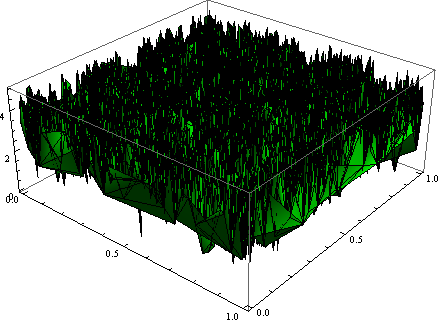
\includegraphics[width=\textwidth]{problem1/my/AEE/18}
			 	 \end{column}
			     \begin{column}{0.3\textwidth}
			     	\caption*{18-й крок. $N(h) = \nn{19322}$.}
			     \end{column}
		     \end{columns}
		\end{figure}
\end{frame}


\begin{frame}[allowframebreaks]
 	\frametitle<presentation>{Таблиця результатів}

 	\scriptsize{\pgfplotstabletypeset[col sep=comma,%
%
		columns={0,1,2,4,5,6,7,3},
		columns/0/.style={
			column name=\textnumero
		},
		columns/1/.style={
			column name=$N(h)$
		},
		columns/2/.style={
			column name=$M(h)$
		},
		columns/3/.style={
			column name=$\norm{e_h^\prime}$,
			fixed,precision=2
		},
		columns/4/.style={
			column name=$\norm{e_h}$,
			fixed,precision=2
		},
		columns/5/.style={
			column name=$\norm{e}$,
			fixed,precision=2
		},
		columns/6/.style={
			column name=${P[u_h]}$,
			fixed,precision=2
		},
		columns/7/.style={
			column name=$\frac{\norm{e_h}}{\norm{e_h+u_h}}\%$
		},
		every head row/.style={before row=\toprule, after row=\midrule},
		every last row/.style={after row=\bottomrule},
		every nth row={1}{before row=\midrule},
		column type/.add={|}{|}
	]{include/8NumResults/problem1/my/errors/table.csv}
}

	\footnotesize{\begin{equation*}
		P[u_h]_i = 2\frac{\ln{\norm{e_h^{i-1}}}-\ln{\norm{e_h^i}}}{\ln{N_i}-\ln{N_{i-1}}} \text{ - показник збіжності.}
	\end{equation*}}


\end{frame}

\begin{frame}{Збіжність похибок}
	\begin{figure}[H]
		\centering
	    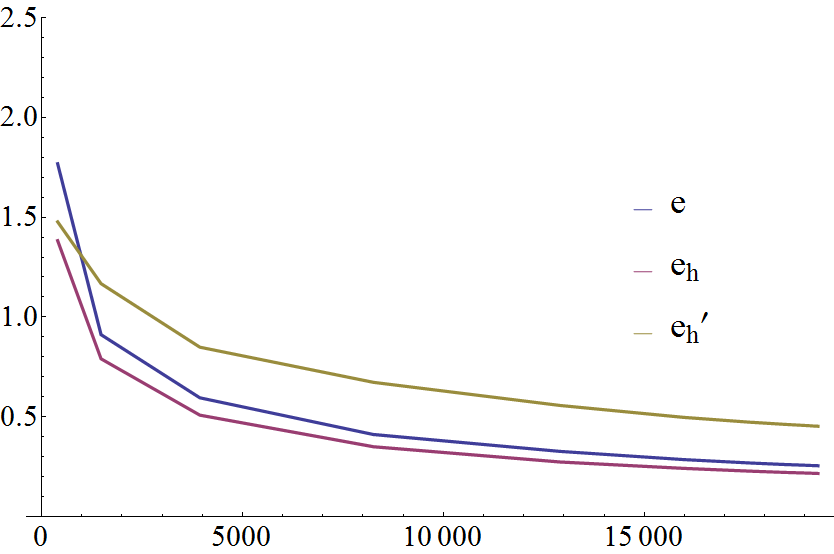
\includegraphics[height=0.8\textheight]{problem1/my/Plotnb}
	    \label{fig:p1_my_errors}
	\end{figure}
\end{frame}

\begin{frame}{З оцінювачем Остапова-Шинкаренка}
	Якщо основу для адаптації беремо $e_h^\prime$

	\scriptsize{\pgfplotstabletypeset[col sep=comma,
		columns={0,1,2,3,5,6,7,4},
		columns/0/.style={
			column name=\textnumero
		},
		columns/1/.style={
			column name=$N(h)$
		},
		columns/2/.style={
			column name=$M(h)$
		},
		columns/3/.style={
			column name=$\norm{e_h^\prime}$,
			fixed,precision=4
		},
		columns/4/.style={
			column name=$\norm{e_h}$,
			fixed,precision=4
		},
		columns/5/.style={
			column name=$\norm{e}$,
			fixed,precision=4
		},
		columns/6/.style={
			column name=${P[u_h]}$,
			fixed,precision=2
		},
		columns/7/.style={
			column name=$\frac{\norm{e_h^\prime}}{\norm{e_h^\prime+u_h}}\%$
		},
		every head row/.style={before row=\toprule, after row=\midrule},
		every last row/.style={after row=\bottomrule},
		every nth row={1}{before row=\midrule},
		column type/.add={|}{|}
	]{include/8NumResults/problem1/ost/errors/table.csv}}

\end{frame}

\begin{frame}{Збіжність похибок}
	\begin{figure}[H]
	 	\centering
	    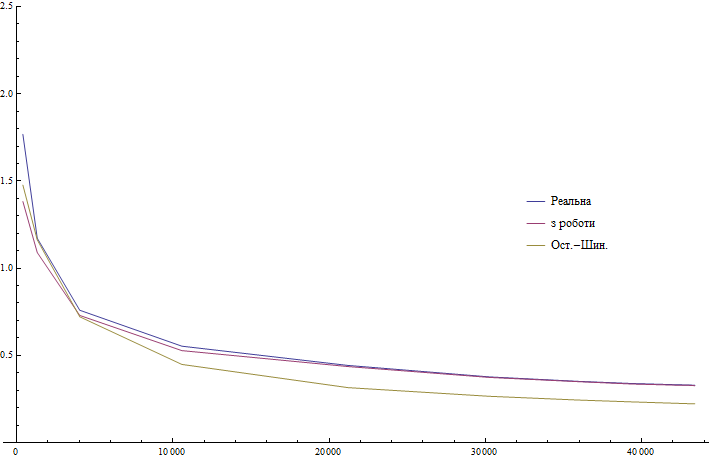
\includegraphics[width=0.8\textwidth]{problem1/ost/Plotnb}
	 \end{figure}
\end{frame}
